\section{Linked Lists}
\label{sec:linked_lists}

\begin{frame}
	\frametitle{Linked list}
	\begin{center}
		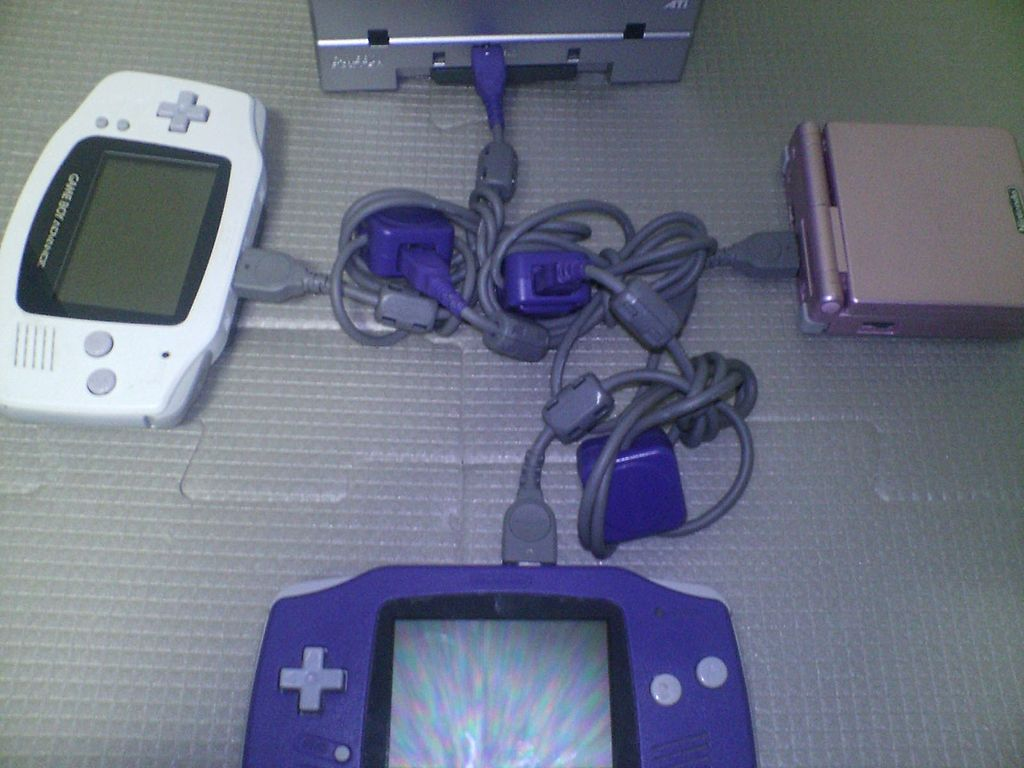
\includegraphics[width=0.6\textwidth]{figures/gba.jpg}\\
		\hspace*{15pt}\hbox{\scriptsize Image By:\thinspace{\itshape PiaCarrot}}
		%https://commons.wikimedia.org/wiki/File:GBA_4PConnection.jpg
	\end{center}
\end{frame}

\begin{frame}
	\frametitle{Another approach}
	
	\begin{problemblock}{What do we want to solve?}
		Two things in the array-based implementation that we hope to solve:
		\begin{enumerate}
			\item Only use space for items we actually use.
			\item Allow for efficient ($O(1)$?) adding and removing at the front of the list.
		\end{enumerate}
	\end{problemblock}
	\pause
	\begin{questionblock}{}
		Why do we want this efficient adding/removing?
	\end{questionblock}
\end{frame}

\begin{frame}
	\frametitle{The notion of a linked list}
	\begin{columns}
		\column{0.455\textwidth}
			\begin{itemize}
				\item We build a list of blocks, starting with one item/block (we call this the \alert{head})
				\item<2-> We can then add another.
				\item<3-> These are connected, we can go from the first to the second item.
				\item<4-> So let's add one more item.
				\item<5-> We should also indicate when we have reached the end (we call this the \alert{tail}).
			\end{itemize}
		\column{0.455\textwidth}
		% Tikz template taken from: https://tex.stackexchange.com/a/19288
\begin{tikzpicture}[list/.style={draw}]

  \node[list] (A) {42};
	\only<2->{
  \node[list] (B) {99};
}
	\only<3->{
  \draw[] let \p1 = (A.two), \p2 = (A.center) in (\x1,\y2) -- (B);
}
	\only<4->{
  \node[list] (C) {12};
  \draw[] let \p1 = (B.two), \p2 = (B.center) in (\x1,\y2) -- (C);
}
\only<5->{
  \node[draw,inner sep=6pt] (D) {};
  \draw (D.north east) -- (D.south west);
  \draw (D.north west) -- (D.south east);
  \draw[] let \p1 = (C.two), \p2 = (C.center) in (\x1,\y2) -- (D);
}
\end{tikzpicture}	

	\end{columns}
\end{frame}

\begin{frame}
	\frametitle{How does this work now?}
	\framesubtitle{Searching for an item}	
	The approach:
	\begin{enumerate}
		\item Start at the head of the list.
		\item<2-> If this is is the item we need, return True.
		\item<2-> Else if this is the tail, return False.
		\item<3-> Else, move to the next item of the list and go to step 2.
	\end{enumerate}

		% Tikz template taken from: https://tex.stackexchange.com/a/19288
\begin{tikzpicture}[list/.style={draw}]

	\node[list,on chain,onslide=<1-2>{red}] (A) {42};
	\node[list,on chain,onslide=<3>{red}] (B) {99};
  \draw[] let \p1 = (A.two), \p2 = (A.center) in (\x1,\y2) -- (B);
  \node[list,on chain,onslide=<4>{red}] (C) {12};
  \draw[] let \p1 = (B.two), \p2 = (B.center) in (\x1,\y2) -- (C);
	\node[on chain,draw,inner sep=6pt,onslide=<5>{red}] (D) {};
	\draw[onslide=<5>{red}] (D.north east) -- (D.south west);
	\draw[onslide=<5>{red}] (D.north west) -- (D.south east);
  \draw[] let \p1 = (C.two), \p2 = (C.center) in (\x1,\y2) -- (D);
\end{tikzpicture}	

	
	\only<6->{
	\lstinputlisting{code/ll_search.py}
}
\end{frame}

\begin{frame}
	\frametitle{Getting an item!?}
	\framesubtitle{Getting item at index $i$}

	\begin{itemize}
		\item There is no easy way to access the $i$th item other than to `walk' there.
		\item So $O(\textit{index})$ to get the item at a certain \texttt{index}.
	\end{itemize}
	\lstinputlisting{code/ll_get.py}
\end{frame}

\begin{frame}
	\frametitle{Inserting at the head or tail}
	\begin{itemize}
		\item Take the current head or tail.
		\item And put the new node before or after it :)
		\item<4-> \alert{$O(1)$ time!}
	\end{itemize}	
	\begin{columns}[t]
		\column{0.535\textwidth}
	\only<2->{
		\lstinputlisting{code/ll_prepend.py}
	}
		\column{0.535\textwidth}
	\only<3->{
		\lstinputlisting{code/ll_append.py}
	}
			
	\end{columns}
\end{frame}

\begin{frame}
	\frametitle{Assumptions, Assumptions}
	\begin{alertblock}{Unfortunately}
		To do \texttt{add\_last} in constant time, we need a reference to the \texttt{tail}.\\
		Many implementations of Singly-Linked Lists do not have this.
	\end{alertblock}		
	\pause
	\begin{questionblock}{Wait Singly?}
		What do I mean with `Singly' Linked List?	
	\end{questionblock}
	\pause
	\begin{answerblock}{Well, it's not doubly linked}
		In other implementations, we can both go forwards and backwards!	
	\end{answerblock}
\end{frame}

\begin{frame}
	\frametitle{Doubly-Linked Lists}
	\begin{overlayarea}{\textwidth}{0.5\textheight}
		\begin{center}
			% Tikz template taken from: https://tex.stackexchange.com/a/19288
\begin{tikzpicture}[list/.style={rectangle split, rectangle split parts=2,
    draw, rectangle split horizontal}, >=stealth, start chain]

  \node[list,on chain] (A) {42};
  \node[list,on chain] (B) {99};
  \draw[*->] let \p1 = (A.two), \p2 = (A.center) in (\x1,\y2) -- (B);
  \node[list,on chain] (C) {12};
  \draw[*->] let \p1 = (B.two), \p2 = (B.center) in (\x1,\y2) -- (C);
  \node[on chain,draw,inner sep=6pt] (D) {};
  \draw (D.north east) -- (D.south west);
  \draw (D.north west) -- (D.south east);
  \draw[*->] let \p1 = (C.two), \p2 = (C.center) in (\x1,\y2) -- (D);

\end{tikzpicture}	

		\end{center}
		\only<1->{
			\begin{block}{A singly linked list}
				Only has connections in one direction.	
			\end{block}	
		}
		\only<2>{
			\begin{center}
				% Tikz template taken from: https://tex.stackexchange.com/a/19288
\begin{tikzpicture}[list/.style={rectangle split, rectangle split parts=2,
    draw, rectangle split horizontal},start chain]

		\only<2->{
  \node[on chain,draw,inner sep=6pt] (E) {};
  \draw (E.north east) -- (E.south west);
  \draw (E.north west) -- (E.south east);
}
  \node[list,on chain] (A) {42};
  \node[list,on chain] (B) {99};
  \draw[*->] let \p1 = (A.two), \p2 = (A.center) in (\x1,\y2) -- (B);
  \node[list,on chain] (C) {12};
  \draw[*->] let \p1 = (B.two), \p2 = (B.center) in (\x1,\y2) -- (C);
  \node[on chain,draw,inner sep=6pt] (D) {};
  \draw (D.north east) -- (D.south west);
  \draw (D.north west) -- (D.south east);
  \draw[*->] let \p1 = (C.two), \p2 = (C.center) in (\x1,\y2) -- (D);

	\only<2->{
		\draw[->,red,thick] let \p1 = (A.two), \p2 = (A.center) in (B) to [out=150, in=30] (\x1,\y2);
		\draw[->,red,thick] let \p1 = (B.two), \p2 = (B.center) in (C) to [out=150, in=30] (\x1,\y2);
		\draw[->,red,thick] let \p1 = (E.center), \p2 = (E.center) in (A) to [out=150, in=30] (\x1,\y2);
	}
\end{tikzpicture}	

			\end{center}
			\begin{block}{A doubly linked list}
				Has connections in both directions.
			\end{block}
		}
	\end{overlayarea}
\end{frame}

\begin{frame}
	\frametitle{Inserting an item}
	\framesubtitle{What to do?}
	\begin{columns}
		\column{0.255\textwidth}
	\begin{itemize}
		\item Navigate to the place where we want to insert the item ($O(\textit{index})$)
			\pause
		\item Add the item: $O(1)$
			\pause
		\item So $O(\textit{index})$ time!
	\end{itemize}
			
		\column{0.755\textwidth}
		\pause
	\lstinputlisting{code/ll_insert.py}
			
	\end{columns}
\end{frame}

\begin{frame}
	\frametitle{Removing an item}
	\begin{questionblock}{Removing an item}
		What is the time complexity of removing the first and last item in a singly linked list?
		\only<1>{
		\begin{enumerate}[A.]
			\item $O(1)$ for the first, $O(1)$ for the last.
			\item $O(1)$ for the first, $O(n)$ for the last.
			\item $O(n)$ for the first, $O(1)$ for the last.
			\item $O(n)$ for the first, $O(n)$ for the last.
			\item I don't know.
		\end{enumerate}
	}
	\end{questionblock}
	\vspace{-20pt}
	\begin{columns}[t]
		
		\column{0.535\textwidth}
	\only<2->{
		\lstinputlisting{code/ll_remove_first.py}
	\vspace{-5pt}
		$O(1)$ time.
	}
		\column{0.535\textwidth}
	\only<3->{
		\lstinputlisting{code/ll_remove_last.py}
	\vspace{-5pt}
		$O(n)$ time.
	}
	\end{columns}
	
\end{frame}

\begin{frame}
	\frametitle{Improvements!}
		\begin{exampleblock}{Doubly-linked list remove last}
			Note that in a doubly-linked list we can remove the last item in $O(1)$ time!\\
			We can just use \texttt{tail.prev} to find the last-but-one element in constant time!\\
		\end{exampleblock}	
\end{frame}

\begin{frame}
	\frametitle{So to summarise}
\begin{columns}
	\column{0.655\textwidth}
	\begin{tabular}{l | c | c | c}
	Operation & Array-based list & SLL & DLL \\	
	\midrule
	Get element $k$ & $O(1)$ &$O(k)$ & $O(k)$ \\
	\pause
	Insert first element& $O(n)$ & $O(1)$ & $O(1)$\\
	Insert at index $k$& $O(n-k)$ & $O(k)$ & $O(\min(k,n-k))$\\
	Append (amortised)& $O(1)$ & $O(1)$ & $O(1)$\\
	\pause
	Remove first element& $O(n)$ & $O(1)$ & $O(1)$\\
	Remove last element& $O(1)$ & $O(n)$ & $O(1)$\\
	Remove index $k$& $O(n-k)$ & $O(k)$ & $O(\min(k,n-k))$\\
	\pause
	Search & $O(n)$ & $O(n)$ & $O(n)$\\
	\end{tabular}
		
	\column{0.355\textwidth}
%	\pause
%	\begin{questionblock}{Which should you use?}
%		So which is better?	
%	\end{questionblock}
%	\pause
%	\begin{answerblock}{It depends!}
%		But on what?	
%	\end{answerblock}
		
\end{columns}

\end{frame}

